%\documentclass[11pt]{article}
\documentclass[preprintnumbers,prd,superscriptaddress,notitlepage,nofootinbib] {revtex4-1}

\usepackage{geometry, amsmath, amsthm, latexsym, amssymb, graphicx,wasysym}
\usepackage[dvipsnames]{xcolor}
\geometry{margin=1in, headsep=0.25in}

% define units, short-names...

\newcommand{\frachalf}{\frac{1}{2}}
\newcommand{\dzbar}{\delta_{\bar{z}}}
\newcommand{\fNL}{f_{\rm NL}}
\newcommand{\kNL}{k_{\rm NL}}
\newcommand{\FoM}{{\rm FoM}}
\newcommand{\cm}{\ \text{cm}}
\newcommand{\pc}{\ \text{pc}}
\newcommand{\Mpc}{\ \text{Mpc}}
\newcommand{\Gpc}{\ \text{Gpc}}
\newcommand{\kpc}{\ \text{kpc}}
\newcommand{\Gyr}{\ \text{Gyr}}
\newcommand{\hkpc}{\ h^{-1}\text{kpc}}
\newcommand{\hMpc}{\ h^{-1}\text{Mpc}}
\newcommand{\hMpcc}{\ h^{-3}\text{Mpc}^3}
\newcommand{\hGpc}{\ h^{-1}\text{Gpc}}
\newcommand{\hGpcc}{\ h^{-3}\text{Gpc}^3}
\newcommand{\ihMpc}{\ h\text{Mpc}^{-1}}
\newcommand{\iMpc}{\ \text{Mpc}^{-1}}
\newcommand{\Ms}{\ M_\odot}
\newcommand{\hMs}{\ h^{-1} M_\odot}
\newcommand{\eh}[1]{\exp{\left[#1\right]}}
\newcommand{\tim}[1]{\times 10^{#1}}%times 10 
\newcommand{\unit}[1]{\ \text{#1}}
\newcommand{\tb}[1]{\textcolor{blue}{#1}}
\newcommand{\tr}[1]{\textcolor{red}{#1}}
\newcommand{\tsc}[1]{#1}
\newcommand{\derd}{\,\mathrm{d}} % upright d for derivatives and integrals
\newcommand{\ddir}{\delta^\text{(D)}}
\newcommand{\dkron}{\delta^\text{(K)}}
\newcommand{\be}{\begin{equation}}
\newcommand{\ee}{\end{equation}}
\newcommand{\la}{\left\langle}
\newcommand{\ra}{\right\rangle}
\newcommand{\derivd}{\text{d}}
\renewcommand{\vec}{\bm}
\newcommand{\FT}[1]{{\rm FT}\left[#1\right]}
\newcommand{\twopicub}{\left(2\pi\right)^3}
\newcommand{\intvkop}{\int\frac{\derivd^3k}{\twopicub}}
\newcommand{\intvx}{\int \derivd^3x~}
\newcommand{\dqc}{\frac{\derivd^3q}{(2\pi)^3}}
\newcommand{\intvqop}{\int \dqc}
\newcommand{\dkpc}{\frac{\derivd^3k'}{(2\pi)^3}}
\newcommand{\dqcp}{\frac{\derivd^3q'}{(2\pi)^3}}
\newcommand{\dqcpp}{\frac{\derivd^3q''}{(2\pi)^3}}
\newcommand{\cyc}{\, \text{cyc.}}
\newcommand{\Dz}{\Delta z}
\newcommand{\Dv}{\Delta v}
\newcommand{\Dx}{\Delta x}
\newcommand{\Deta}{\Delta \eta}
\newcommand{\Dtheta}{\Delta \theta}
\newcommand{\bz}{\bar{z}}
\newcommand{\kms}{{\rm km~s^{-1}}}
\newcommand{\ikms}{{\rm s~km^{-1}}}
\newcommand{\kmsMpc}{\nicefrac[\rm]{km}{s\,Mpc}}
\newcommand{\summnu}{\Sigma m_\nu}
\newcommand{\Nnueff}{N_{\nu,{\rm eff}}}
\newcommand{\kmaxeff}{k_{\rm max,eff}}
\newcommand{\kmax}{{k_{\rm max}}}
\newcommand{\kmin}{{k_{\rm min}}}
\newcommand{\kNyq}{{k_{\rm Nyq}}}
\newcommand{\neff}{{n_{\rm eff}}}
\newcommand{\sL}{\mathcal{L}}
\newcommand{\sN}{\mathcal{N}}
\newcommand{\sH}{\mathcal{H}}
\newcommand{\sD}{\mathcal{D}}
\newcommand{\gmunu}{{g_{\mu \nu}}}
\newcommand{\keV}{{\rm keV}}
\newcommand{\GeV}{{\rm GeV}}
\newcommand{\erg}{\, {\rm erg}}
\newcommand{\gram}{\, {\rm g}}
\newcommand{\kelvin}{\, {\rm K}}
\newcommand{\deltahat}{\hat{\delta}}

%bias parameters
\newcommand{\bdelta}{b_\delta}
\newcommand{\bdtwo}{b_{\delta^2}}
\newcommand{\bstwo}{b_{s^2}}
%renormalized fields
\newcommand{\msdtwo}{\left[\delta^2\right]}
\newcommand{\msstwo}{\left[s^2\right]}
%bold faced vectors
\newcommand{\vtheta}{\mathbf{\theta}}
\newcommand{\vDtheta}{\mathbf{\Delta \theta}}
\newcommand{\vv}{\mathbf{v}}
\newcommand{\vnabla}{\mathbf{\nabla}}
\newcommand{\veta}{\mathbf{\eta}}
\newcommand{\vk}{\mathbf{k}}
\newcommand{\vq}{\mathbf{q}}
\newcommand{\vt}{\mathbf{t}}
\newcommand{\vb}{\mathbf{b}}
\newcommand{\vx}{\mathbf{x}}
\newcommand{\vc}{\mathbf{c}}
\newcommand{\vone}{\mathbf{1}}
\newcommand{\vmu}{\mathbf{\mu}}
\newcommand{\vzeta}{\mathbf{\zeta}}
\newcommand{\vn}{\mathbf{n}}
\newcommand{\vgamma}{\mathbf{\gamma}}
\newcommand{\vpi}{\mathbf{\pi}}
\newcommand{\vrho}{\mathbf{\rho}}
\newcommand{\vphi}{\mathbf{\phi}}
\newcommand{\vchi}{\mathbf{\chi}}
\newcommand{\vomega}{\mathbf{\omega}}
\newcommand{\vu}{\mathbf{u}}
\newcommand{\vj}{\mathbf{j}}
\newcommand{\vg}{\mathbf{g}}
\newcommand{\vm}{\mathbf{m}}
\newcommand{\vd}{\mathbf{d}}
\newcommand{\vdelta}{\mathbf{\delta}}
\newcommand{\vy}{\mathbf{y}}
\newcommand{\vf}{\mathbf{f}}
\newcommand{\vp}{\mathbf{p}}
\newcommand{\vep}{\mathbf{\epsilon}}
\newcommand{\vo}{\mathbf{o}}
\newcommand{\vs}{\mathbf{s}}
\newcommand{\vsh}{\hat{\mathbf{s}}}
\newcommand{\vS}{\mathbf{S}}
\newcommand{\vC}{\mathbf{C}}
\newcommand{\vXi}{\mathbf{\Xi}}
\newcommand{\vQ}{\mathbf{Q}}
\newcommand{\vDelta}{\mathbf{\Delta}}
\newcommand{\vP}{\mathbf{P}}
\newcommand{\vN}{\mathbf{N}}
\newcommand{\vA}{\mathbf{A}}
\newcommand{\vM}{\mathbf{M}}
\newcommand{\vK}{\mathbf{K}}
\newcommand{\vB}{\mathbf{B}}
\newcommand{\vU}{\mathbf{U}}
\newcommand{\vT}{\mathbf{T}}
\newcommand{\vF}{\mathbf{F}}
\newcommand{\br}{\mathbf{r}}
\newcommand{\vR}{\mathbf{R}}
\newcommand{\Tr}{\mathrm{Tr}}
\newcommand{\lnL}{{\mathcal{L}}}
\newcommand{\vxperp}{\mathbf{x_\perp}}
\newcommand{\vkperp}{\mathbf{k_\perp}}
\newcommand{\kperp}{k_\perp}
\newcommand{\vrperp}{\mathbf{r_\perp}}
\newcommand{\vpar}{v_\parallel}
\newcommand{\rpar}{r_\parallel}
\newcommand{\kpar}{k_\parallel}
\newcommand{\tk}{\tilde{k}}
\newcommand{\tmu}{\tilde{\mu}}
\newcommand{\PtD}{P_{\rm 3D}}
\newcommand{\PtDp}{P_{\rm 3D^\prime}}
\newcommand{\vPsi}{\mathbf{\Psi}}
\newcommand{\vUpsilon}{\mathbf{\Upsilon}}
\newcommand{\vV}{\mathbf{V}}
\newcommand{\vW}{\mathbf{W}}
\newcommand{\vrhat}{\mathbf{\hat{r}}}
\newcommand{\vxhat}{\mathbf{\hat{x}}}
\newcommand{\vzhat}{\mathbf{\hat{z}}}
\newcommand{\vz}{\mathbf{z}}
\newcommand{\vpsi}{\mathbf{\psi}}
\newcommand{\vupsilon}{\mathbf{\upsilon}}
\newcommand{\bn}{\bar{n}}
\newcommand{\rhobar}{\bar{\rho}}
\newcommand{\vI}{\mathbf{I}}
\newcommand{\vH}{\mathbf{H}}
\newcommand{\vl}{\mathbf{l}}
\newcommand{\vL}{\mathbf{L}}
\newcommand{\vG}{\mathbf{G}}
\newcommand{\vD}{\mathbf{D}}
\newcommand{\vE}{\mathbf{E}}

%LyaF
%removed \ after several here - makes space before period - 
%add by hand when needed
\newcommand{\lya}{Ly$\alpha$}
\newcommand{\lyb}{Ly$\beta$}
\newcommand{\lyaf}{Ly$\alpha$ forest}
\newcommand{\vdf}{{\mathbf \delta_f}}
\newcommand{\vdF}{{\mathbf \delta_F}}
\newcommand{\lr}{\lambda_{{\rm rest}}}
\newcommand{\PF}{$P_F^{\rm 1D}(k_\parallel,z)$}
\newcommand{\bF}{\bar{F}}
\newcommand{\bC}{\bar{C}}
\newcommand{\bT}{\bar{T}}
\newcommand{\bS}{\bar{S}}

%journals
\newcommand{\mnras}{{\em Mon. Not. Roy. Astron. Soc. }}
\newcommand{\apjl}{{\em Astrophys. J. Let. }}
\newcommand{\apjs}{ApJS}
\newcommand{\jcap}{JCAP}
\newcommand{\physrep}{{\em Phys. Rept. }}
\newcommand{\aap}{{\em Astron. Astrophys. }}
\newcommand{\aj}{AJ }
\newcommand{\pasp}{PASP}
\newcommand{\pasj}{PASJ}
\newcommand{\uros}{Uro\v{s}}
\newcommand{\anze}{An\v{z}e}

\def\prd{{\em Phys. Rev. }{\bf D }}
\def\pr{{Phys.\ Rev.\ }}
\def\astropart{{Astro-particle Phys.~}}
\def\rvmp{{Rev.\ Mod.\ Phys.\ }}

\def\pvm#1{[PM: {\it #1}] }
\def\pvmhid#1{}
\def\af#1{[AF: {\it #1}] }
\def\afhid#1{}
\def\as#1{[AS: {\it #1}] }
\def\ashid#1{}
\def\hs#1{[HS: {\it #1}] }
%vb conflicts with \vb = \mathbf{b} used elsewhere
\def\vbh#1{[VB: {\it#1}] }
\def\cs#1{[CS: {\it#1}] }
\def\sb#1{[SB: {\it #1}] }
\def\zs#1{[ZS: {\it #1}] }
\def\zv#1{[ZV: {\it #1}] }
\def\uscomment#1{[US: {\it #1}] }
\def\referee#1{[REFEREE: {\it#1}] }


\newcommand{\afr}[1]{{\color{red}AFR: #1}}
\newcommand{\as}[1]{{\color{blue}AS: #1}}
\newcommand{\pvm}[1]{{\color{olive}PVM: #1}}

%Silence comments
\def\afrhid#1{}
%\newcommand{\afrhid}[1]{{\color{red}AFR: #1}}
%\def\ashid#1{}
\newcommand{\ashid}[1]{{\color{blue}AS: #1}}
%\def\pvmhid#1{}
\newcommand{\pvmhid}[1]{{\color{olive}PVM: #1}}
\newcommand{\CP}[1]{{\color{red}CP: #1}}
\newcommand{\fluxpower}{$P_\mathrm{1D}(k_\parallel)$}
\newcommand\LCDM{$\Lambda$CDM}

\def\todo#1{[TO DO: {\it #1}] }



\begin{document}

\title{Parameterisation of \lya\ forest likelihoods}

\author{Chris Pedersen} % \footnote{author list alphabetized}}
\email{chrisp@star.ucl.ac.uk} 
\affiliation{Department of Physics and Astronomy, University College London, 
Gower Street, London, United Kingdom}

\date{\today}

\begin{abstract}
In this short internal note we discuss different sets of likelihood parameters
we could use in our emulator, and ways in which we could interface our emulator
with other cosmological probes. We propose a likelihood parameterisation around
the amplitude and slope of the linear power spectrum in velocity units as
presented in ref \cite{McDonald2005a}, and propose a test to demonstrate that
all the cosmologically relevant information in the \lyaf\ is contained within
these parameters.
\end{abstract}

\maketitle

\section{Introduction}
One of the novelties in the construction of our emulator when compared with
previous approaches is the use of different parameter spaces in different parts
of the emulator. A motivation for this is to avoid using parameters that are
highly degenerate with one another. The \lyaf\ is
sensitive to the matter power spectrum in a small redshfit ($2<z<5$) and
$k$ ($0.1\lessapprox k \lessapprox 10 \iMpc $) range, and when considering only
this regime, the effects of $\Lambda$CDM$\nu$ parameters are strongly degenerate with
one another\cite{Pedersen2020}. The effects of changing these parameters on the flux statistics are also
often degenerate with changes to the intergalactic medium (IGM). In this redshift
range, the universe is also very close to Einstein de-Sitter, so the dependence of the
growth factor and the expansion rate are close to indepenent of cosmological model.
Previous studies have interpolated the \fluxpower\ as a function of parameters
such as $H_0$, $\Sigma_\nu$, $\Omega_m$\cite{Yeche2017},
however the effect of changing these
parameters on the \fluxpower\ occurs through changing the matter clustering
as described by the power spectrum, and changing the IGM.
Given that ultimately one would want to marginalise over the IGM,
training the emulator on these highly degenerate parameters is not
optimal.
So we instead parameterise our emulator directly on the linear power, using a set of
parameters that are more orthogonal to one another and closer to the data which should
result in more reliable predictions, and more robust constraints.

In addition to using a reduced and more orthogonal set of parameters, this approach also
provides a model-independent emulator that can be used in joint constraints of
extended models, such as curvature, non-standard $N_\mathrm{eff}$, and time-varying
dark energy without these models needing to be included in the original emulator.
First in section \ref{sec:emu_space} we cover the emulator parameter space in closer
detail, and describe how our emulator can be combined with analysis of the CMB.
Then in section \ref{sec:compressed} we discuss ways to simplify this procedure
so that users do not need to run the emulator code and marginalise over the IGM
in order to use \lyaf\ results.

\afrhid{In my opinion, there are two different discussions that we should not mix:
\begin{itemize}
 \item (A) Why the emulator works with linear power parameters instead of working with cosmological parameters.
 \item (B) Why do we want to present a marginalised likelihood in terms of linear power parameters (in velocity units).
 \end{itemize}
There are different motivations for (A), but I think the most important one is that this allows us to run cosmological analyses in non-\LCDM\ models, even if the emulator was constructed using only \LCDM\ simulations. I'm thinking of the usual extensions that people discuss, like open curvature, non-zero neutrino masses, $w$CDM models, and so on. 
It would be really hard to train an emulator that had all these parameters as labels.
For (B), the motivation is so that we can provide a light-weight and fast likelihood module that
others can use.
However, it is important to differentiate (A) from (B), since if we didn't want to provide any
marginalised / compressed likelihood, we would still want the emulator to work with linear
power parameters.}



\section{Emulator parameter space}
\label{sec:emu_space}
We have opted to train our emulator to predict a \fluxpower\ as
a function of the linear matter power spectrum, which we have parametrised in
terms of an amplitude and a slope around a small scale pivot:

\begin{equation}
    \label{eq:Delta2_p}
    \Delta^2_p(z)=k^3P(k, z)/2\pi^2|_{k=k_\star}
\end{equation}

%\afr{Minor point, but there are $2 \pi$ factors in the definition of $\Delta$}

\begin{equation}
    \label{eq:n_p}
    n_p(z)=d\rm{ln}P(k,z) / d \rm{ln}(k)|_{k=k_\star}
\end{equation}

where $P(k,z)$ is the linear CDM + baryon power spectrum, and we set the pivot
scale $k_\star=0.69 \iMpc$. We also use $4$ nuisance parameters
to describe the IGM:

\begin{itemize}
    \item $\langle F \rangle$, the mean flux,
    \item $\sigma_T$, the temperature at mean density of the IGM,
    \item $\gamma$, quantifying how the temperature scales with density,
    \item $k_F$, the pressure smoothing scale.
\end{itemize}

We train one Gaussian
process on all snapshots from all simulations in a given suite to predict a
comoving \fluxpower\ as a function of these $6$ parameters, which we refer to as the
emulator parameters. One benefit of this approach is that the emulator can be used
to create theoretical predictions for data at any redshift within the range where
we have training data, meaning that the snapshot outputs of our training simulations
does not need to match the redshift binning of future or past surveys.
Training simulations with different snapshot outputs can also in principle be combined
to form bolstered training sets.

In Fig \ref{fig:param_map1} we show how our emulator could be combined with
CMB likelihoods. At each cosmological model in the Planck chain, a \textsc{CAMB}
object is used to calculate the emulator parameters $\Delta^2_p(z)$ and $n_p(z)$
at each redshift where we have data. This results in $N$ emulator calls, where $N$
is the number of data redshift bins. The emulated \fluxpower\ is then converted
into velocity units using the factor $H(z)/1+z$ calculated from
the \textsc{CAMB} model. The log likelihood for this given model is then calculated
from the data. NB that for brevity we do not discuss the details of modelling or
marginalisation of the IGM in this document, for now let's imagine that the last
step in this process would involve some marginalisation procedure.

\begin{figure}[ht]
    \begin{center}
     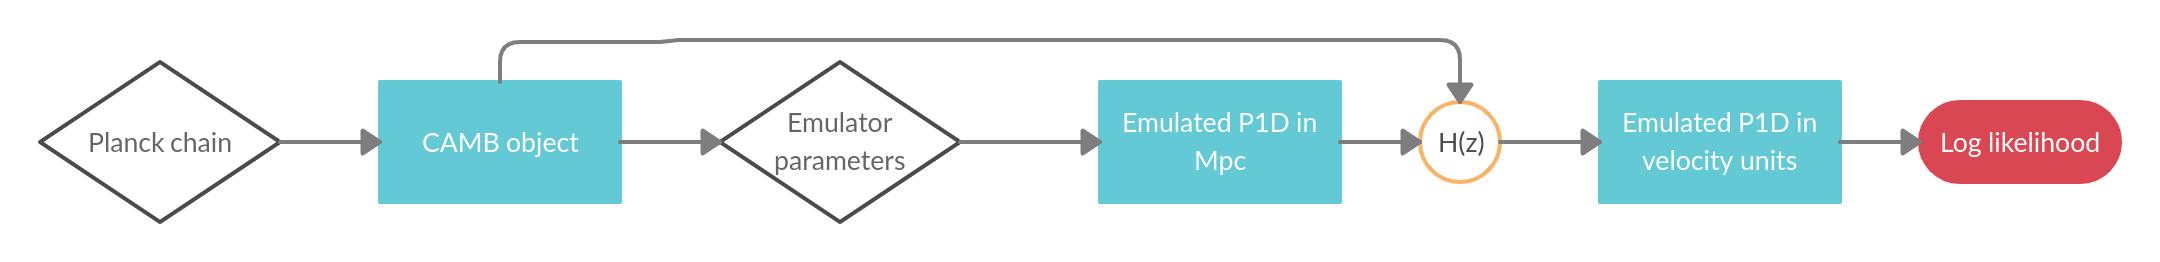
\includegraphics[scale=0.2]{Figures/Parameter_mapping.png}
    \end{center}
    \caption{Procedure for evaluating a \lyaf\ likelihood for a given
    point in the Planck chain.
    For each cosmological
    model, a \textsc{CAMB} object is created, and the emulator parameters defined
    in equations \ref{eq:Delta2_p} and \ref{eq:n_p} are calculated, for each redshift $z$.
    The $H(z)$ calculated
    for each model is then used to convert the comoving emulated \fluxpower\
    to velocity units, and a log likelihood is calculated.}
    \label{fig:param_map1}
\end{figure}



\section{Compressed likelihood parameters}
\label{sec:compressed}
The approach shown in Fig \ref{fig:param_map1} requires the user to run the emulator
code and marginalise over the IGM. This requires expertise and is computationally slow,
and so while this is appropriate for our first tests of the emulator, it is worthwhile to
consider more practical ways which would allow a wider set of users to be able to
incorporate \lyaf\ results in their constraints. We propose to follow
the approach presented in \cite{McDonald2005a}, and parameterise our likelihood
in terms of the small scale linear power in velocity units:

\begin{equation}
    \label{eq:Delta2_star}
    \Delta^2_\star=q^3P(q, z)/2\pi^2|_{q=q_\star,z=z_\star}
\end{equation}

\begin{equation}
    \label{eq:n_star}
    n_\star=d\rm{ln}P(q,z) / d \rm{ln}(k)|_{q=q_\star,z=z_\star}
\end{equation}

where $q$ refers to a wavenumber in velocity units, and we set a pivot
redshift of $z_\star=3$ and $q_\star=0.009$ s/km.\footnote{Note that this pivot
scale can be chosen independently to $k_\star$ used in emulator parameter space.}
We refer to these parameters as the compressed likelihood parameters.
\afrhid{It might be useful to highlight that this pivot point does not need to match the
pivot point in the emulator.}
We note here that when using
only these two parameters we are fixing the growth rate and expansion
history to a fiducial model. One could then present marginalised likelihoods for
these parameters, which could be included in packages like \textsc{MontePython}
and \textsc{CosmoMC}. In this case the \lyaf\ contribution to a joint likelihood
would be found using the procedure shown in Fig \ref{fig:marginalised_compressed}.
Here for a given cosmological model, the compressed likelihood parameters are calculated,
and the \lyaf\ likelihood for this model is looked up in some form of table.

\begin{figure}[ht]
    \begin{center}
     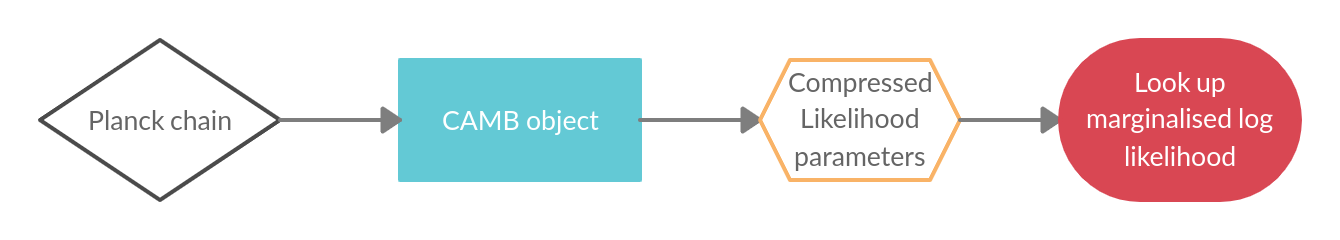
\includegraphics[scale=0.2]{Figures/Marginalised_compressed.png}
    \end{center}
    \caption{Once we have calculated marginalised likelihoods for the compressed
    likelihood parameters, the \lyaf\ likelihood for a given cosmological model
    can simply be looked up.}
    \label{fig:marginalised_compressed}
\end{figure}

It is important to demonstrate that there is no significant loss of information
when compressing the information in the \lyaf\ down to the compressed likelihood
parameters. The way we propose to show this is through the approach show in
Fig \ref{fig:param_test}, which is very similar to the first procedure in Fig
\ref{fig:param_map1}, except that the emulator calls are made having first gone
through the compressed parameters. We intend to compare the combined CMB + \lyaf\
posteriors when calculating the \lyaf\ likelihood using these two different approaches.
If the posteriors are unchanged whether or not the compressed parameters are used,
we will be able to conclude that all the cosmologically relevant information
in the \lyaf\ is contained within the compressed parameters.


\begin{figure}[ht]
    \begin{center}
     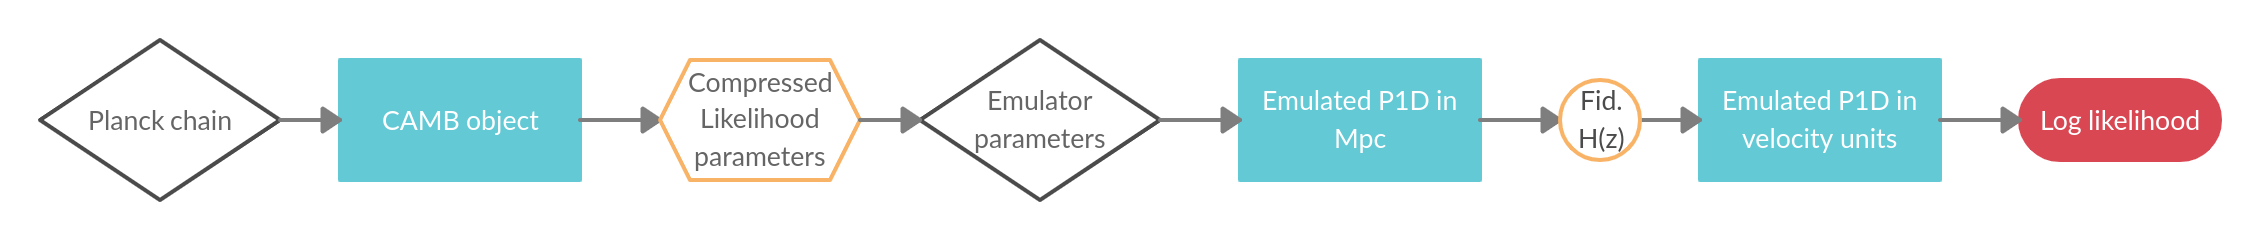
\includegraphics[scale=0.2]{Figures/Compressed_test.png}
    \end{center}
    \caption{Here we evaluate each \lyaf\ likelihood contribution going
    through the compressed likelihood parameters. Instead of calculating
    the emulator calls directly from the cosmological model, the compressed
    likelihood parameters are calculated first, and these are then used to
    find the emulator parameters. A fiducial expansion history is then used for
    the conversion of the emulated \fluxpower\ to velocity units.}
    \label{fig:param_test}
\end{figure}

To what extent our approximations of a fixed fiducial expansion history and
growth rate are valid is a question we are currently working on. There is a physical
argument suggesting we are largely insensitive to these, however we do not know
at what threshold the precision in the data and emulator will break this insensitivity.
We are testing this by introducing some parameters that add freedom in these two
dimensions, which we can go into more detail on in a future discussion.
As a final note it is also trivial to add a running of the spectral index
to the parameter spaces above, and it is worth discussing whether or not we
want to include this in the first paper.

\bibliography{main}
\bibliographystyle{JHEP}

\end{document}
